\documentclass[12pt,oneside]{article}
\usepackage{../../light}
\usepackage{multicol}

\usepackage{pifont} % for the star

\usepackage{palatino}
% No Palatino! It messes up the break in the woodchuck problem, part (b).
% The humor doesn't work as well with the last word of the tongue-twister
% on the second line.

%.... Palatino reinstituted. Wording changes messed up that problem anyway. Oh well.
\usepackage{mathpazo}

\usepackage{verbatim}
\newcommand{\mfigure}[3]{\bigskip\centerline{\resizebox{#1}{#2}{\includegraphics{#3}}}\bigskip}
\newcommand{\hint}[1]{({\it Hint: #1})}
\newcommand{\brule}[1]{\underline{\hspace{#1}}}
\newcommand{\ang}[1]{\left< #1 \right>}
\newcommand{\beats}{\rightarrow}

\newenvironment{falseproof}
{\begin{proof}[False proof]}
{\end{proof}}


\showsolutions
%\hidesolutions


%title for individual problem
\newcommand{\ptitle}[1]{\textbf{\hspace{0.2cm}#1}}


\begin{document}
\generic{Final Exam}{December 17, 2008}

\instatements{
\vspace{24pt}
\textbf{Name:} \rule{5in}{0.5pt}

\textbf{Circle the name of your recitation instructor}:

\begin{center}
\begin{tabular}{lllllll}
Bill & Brooke & Chieu & Jay & Ling & Nick & Spyros 
\end{tabular}
\end{center}


%\begin{multicols}{2}

\begin{itemize}

\item This final is \textbf{closed book}, but you may have three $8.5"
\times 11"$ sheets with notes in your own handwriting on both sides.

\item You may not use a calculator or a Python interpreter, and while exercising skill with a PostScript interpreter 
would highly impress at least one member of the course staff, you are not allowed to use that either.
You \emph{may} work with any of the following: a slide 
rule, an abacus, a Curta, Napier's bones, any original version of the Antikythera mechanism, 
an Enigma machine, and/or the difference engine. You are also permitted to use a perpetual motion machine as a source of 
energy, and an antigravity device to elevate yourself above the rest of the 
class. 


\item You may assume all of the results presented in class.

\item Please show your work.  Partial credit cannot be given for a wrong
answer if your work isn't shown.

\item Write your solutions in the space provided.  If you
need more space, write on the back of the sheet containing the
problem.  Please keep your entire answer to a problem on that
problem's page.

\item Be neat and write legibly.  You will be graded not only on the
correctness of your answers, but also on the clarity with which you
express them.

\item If you get stuck on a problem, move on to others. The problems 
are not arranged in order of difficulty.

\item Please resist the urge to roll on the floor laughing out loud.

%\item The exam ends at 4:30 PM.
\item You have three hours to complete the exam.

\end{itemize}

%\vspace{0.25in}

%\columnbreak

%\vspace*{1in}
%\begin{multicols}{2}

\begin{center}
{\large

\begin{tabular*}{6in}{|l|@{\extracolsep{\fill}}|c|c|c|c|c|c|c|c|c|c|c|}
 \hline
 Problem & 1 & 2 & 3 & 4 & 5 & 6 & 7 & 8 & 9 & 10 & Total \\ \hline
 Points & 25 & 25 & 25 & 15 & 15 & 15 & 25 & 15 & 20 & 20 & 200\\ \hline
 Score & & & & & & & & & & &\\ \hline
 Grader & & & & & & & & & & &\\ \hline
\end{tabular*}
}
\end{center}


%\begin{tabular}{|c|c|c|c|}
%\hline
%Problem & Points & Grade & Grader \\ \hline \hline
%1 & 25 & & \\ \hline
%2 & 25 & & \\ \hline
%3 & 25 & & \\ \hline
%4 & 15 & & \\ \hline
%5 & 15 & & \\ \hline
%\end{tabular}

%\columnbreak

%\begin{tabular}{|c|c|c|c|}
%\hline
%Problem & Points & Grade & Grader \\ \hline \hline

%6 & 15 & & \\ \hline
%7 & 25 & & \\ \hline
%8 & 15 & & \\ \hline
%9 & 20 & & \\ \hline
%10 & 20 & & \\ \hline

%Total & 200 & & \\ \hline
%\end{tabular}
%}
%\end{center}

%\end{multicols}
}



\instatements{\newpage}


% NOTES:
%
% Topics:
% - 1/3 pure probability
% - 1/3 probability combined with earlier topics
% - 1/3 pure earlier topics
%
% - Repeat invariant problem of quiz 1
%
% Problems:







%Ling:
% Straightforward probability, covers the following:
%-Expectation, conditional expectation
%-Total Expectation
%-Variance
%-Markov, Chebyshev, Chernoff

%test techniques:
%using total expectation and conditional expectation
%using functions on random variables to find expectation??
%variance on an indicator variable + linearity when independent
%variance on non-indicator variables
%using the different bounds
\instatements{\newpage}
\begin{problem}{25}\label{probability} \ptitle{The Final Breakdown}

Suppose the 6.042 final consists of:

\begin{itemize}
\item 36 true/false questions worth 1 point each.
\item 1 induction problem worth 15 points.
\item 1 giant problem that combines everything from the semester, worth 49 points.
\end{itemize}

Grading goes as follows:
\begin{itemize}
\item The TAs choose to grade the easy true/false questions. For each individual point, they flip a fair coin. If it comes up heads, the student gets the point.

\item Marten and Brooke split the task of grading the induction problem.
\begin{itemize}
\item With $1/3$ probability, Marten grades the problem. His grading policy is as follows: Either he gets exasperated by the improper use of math symbols and gives 0 points (which happens with $2/5$ probability), or he finds the answer satisfactory and gives 15 points (which happens with $3/5$ probability).
\item With $2/3$ probability, Brooke grades the problem. Her grading policy is as follows: She selects a random integer point value from the range from $0$ to $15$, inclusive, with uniform probability.
\end{itemize}

\item Finally, Tom grades the giant problem. He rolls two fair {\bf seven}-sided dice (which have values from $1$ to $7$, inclusive), takes their product, and subtracts it from 49 to determine the score. (Example: Tom rolls a 3 and a 4. The score is then $49 - 3 \cdot 4 = 37$.)

\end{itemize}

Assume all random choices during the grading process are mutually independent. 

%The next page lists the different problem parts.
The problem parts start on the next page.
Show your work to receive partial credit.

\instatements{\newpage}


\bparts

\ppart{7} What is the expected score on the exam?
\solution[\vspace{5in}]{
 $$ 36/2 + (1/3)15(3/5) + (2/3)15/2 + (49-(4*4))= 18 + 3 + 5 + 33=59$$

The expected score on the exam is the sum of the expected scores on the individual problems.
\[
\ex{\text{test score}} = \ex{\text{mc score}} + \ex{\text{ind score}} + \ex{\text{giant score}}
\]

\begin{itemize}

\item The expected multiple choice score is just the sum of the expectations on 36 coin tosses. Since the coin is fair, the expected number of heads on each flip is 1/2. Therefore:
\[
\ex{\text{mc score}} = 36 \cdot 1/2 = 18
\]

\item The expected induction score is a weighted sum of the expectations on problems graded by Marten and Brooke. Let $M$ be the event that Marten graded the problem, and $B$ be the event that Brooke graded the problem. Therefore:
\begin{align*}
\ex{\text{ind score} \mid M} &= 0 \cdot 2/5 + 15 \cdot 3/5 = 9 \\
\ex{\text{ind score} \mid B} &= \sum_{i=0}^{15} \left( i \cdot 1/16\right) = 15/2
\end{align*}
\begin{align*}
\ex{\text{ind score}} &= \ex{\text{ind score} \mid M} \pr{M} + \ex{\text{ind score} \mid B} \pr{B} \\
&= 9 \cdot 1/3 + 15/2 \cdot 2/3 = 8
\end{align*}

\item The expected giant problem score is the expectation on 49 minus the product of rolls of two fair seven-sided dice. We can pull out the constant 49, and (since the dice are independent) the expectation on the product of the rolls becomes the product of the expectations on the rolls, which is 4 in this case (average of numbers 1 to 7). Therefore, if $R$ is the random variable representing the roll of a single die:
\[
\ex{\text{giant score}} = \ex{49 - R^2} = 49 - \ex{R}^2 =  49 - (4)^2 = 49 - 16 = 33
\]

\end{itemize}

Therefore, the overall expectation is:
\[
\ex{\text{test score}} = 18+8+33 = 59
\]

}

\ppart{5} What is the variance on the 36 true/false questions?
\solution[\vspace{3in}]{
Since the coin flips are independent, we can sum the variances of each flip.
\[
\variance{\text{mc score}} = 36 \cdot 1/2 \cdot 1/2 = 9
\]
}

\ppart{5} What is the variance on the induction score, given that Marten graded the problem? 
\solution[\vspace{2.75in}]{
Using the equation $\variance{X} = \ex{X^2} - \ex{X}^2$:
\[
\variance{\text{ind score}} = (15^2 \cdot 3/5)-(9)^2=135-81=54
\]
}

\ppart{3} Argue why the Markov bound can be used to determine an upper bound on the probability that the score on the exam is $\geq 80$.  You do not need to compute the actual bound.
\solution[\vspace{2.25in}]{
The Markov bound can be used if there is a lower bound on the possible values of the random variable. In this case, all test scores are $\geq 0$.
}

\ppart{5} Use the Chebyshev bound to determine an upper bound on the probability that the score on the true/false questions is $\geq 24$.
\solution[\vspace{2.75in}]{
If $C$ be the random variable representing the multiple choice score:
\begin{align*}
\pr{ C \geq 24 } &\leq \pr{ \mid C - 18\mid \geq 6 } \\
&= \pr{ \mid C - \ex{C}\mid \geq 6 } \\
&\leq \frac{\variance{C}}{6^2} \\
&= \frac{9}{36} = \frac{1}{4}
\end{align*}
}

\eparts


\end{problem}



% Chieu: conditional prob;
\instatements{\newpage}
\begin{problem}{25}\label{woodchuck} \ptitle{Woodchucks Chucking Wood}
%give a set of conditional probabilities, part (a) applies Bayes' rule to get reversed conditional probabilities, part (b) applies incl/excl in order the calculate a probability of a union of events.

All woodchucks can chuck wood, but only some can do it well.
\begin{itemize}
 \item $1/3$ of all woodchucks like to chuck wood.
 \item $2/3$ of all woodchucks can chuck wood well.
 \item $1/2$ of those that like chucking wood can do it well.
 \item The expected amount of wood chucked by a woodchuck (randomly chosen with uniform probability) is $7$ kg/day.
 \item The expected amount of wood chucked by a woodchuck that likes chucking wood but can't do it well is $1$ kg/day.
 \item A woodchuck that does not like chucking wood does not chuck any wood at all, regardless of its wood-chucking skillz or lack thereof.
\end{itemize}


\bparts

\ppart{10} What is the probability that a woodchuck (randomly chosen with uniform probability) likes chucking wood, given that it can do it well?

\solution[\vspace{2in}]{
Let $L$ be the event that a woodchuck likes chucking wood and $C$ be the event that a woodchuck can chuck wood well. We are given:
\begin{align*}
 Pr(L) &= 1/3 \\
 Pr(C) &= 2/3 \\
 Pr(C|L) &= 1/2
\end{align*}
We wish to find $Pr(L|C)$. Using Bayes' rule, we have
\begin{align*}
 Pr(L|C) &= \frac{Pr(C|L)Pr(L)}{Pr(C)} \\
 &= \frac{(1/2)(1/3)}{(2/3)} \\
 &= 1/4
\end{align*}
}


\instatements{\newpage}

\ppart{15} On average, how much wood would a woodchuck chuck if the woodchuck could chuck wood well?
\solution{
Let $W$ be a random variable representing the amount of wood the woodchuck chucks. We are given (in units of kg/day):
\begin{align*}
 E(W) &= 7\\
 E(W|(L\cap \bar U)) &= 1
\end{align*}

Using the law of total expectation, we can partition the sample space into three events: (1) the woodchuck can chuck wood well; (2) the woodchuck can't chuck wood well but likes chucking wood; (3) the woodchuck can't chuck wood well and doesn't like chucking wood.
\begin{align*}
 E(W) &= E(W|C)Pr(C) + E(W|(\bar C\cap L))Pr(\bar C\cap L) + E(W|(\bar C\cap\bar L))Pr(\bar C\cap\bar L) \\
 7 &= E(W|C)(2/3) + 1\cdot Pr(\bar C\cap L) + E(W|(\bar C\cap\bar L))Pr(\bar C\cap\bar L) 
\end{align*}
Since a woodchuck that doesn't like chucking wood does not chuck any wood, whether or not it can do so, $E(W|\bar C\cap\bar L) = 0$, so the last product in the sum vanishes:
\begin{align*}
 7 &= E(W|C)(2/3) + Pr(\bar C\cap L) 
\end{align*}
Finally, from the definition of conditional expection, we have
\begin{align*}
Pr(\bar C\cap L) &= P(\bar C|L)P(L) \\
 &= (1-P(C|L))P(L) \\
 &= (1-1/2)(1/3) \\
 &= 1/6
\end{align*}

We wish to find $E(W|C)$, the expected amount of wood chucked by a woodchuck that can chuck wood well:
\begin{align*}
 7 &= E(W|C)(2/3) + 1/6 \\
 41/6 &= E(W|C)(2/3) \\
 41/4 &= E(W|C)
\end{align*}

So $E(W|C) = 41/4 = 10.25$.

}

\eparts
\end{problem}



%  replace \ding{73} with $\star$ if not using the pifont package
\newcommand{\kstar}{\ding{73}}

%  Tom's 3-player card game
\instatements{\newpage}
\begin{problem}{25}\label{cards} \ptitle{Cardsharing\kstar Revolution}

Three 6.042 students---Kirari, Noelle, and Cobeni---are
 playing a game of Tan Tan Taan!.  During each round of Tan Tan Taan!, 
each player is dealt 4 cards of their own, and one additional card is shared among all  players, so that each
player has 5 cards that they can use (the 4 cards of their own along with the single shared card).
  Cards are uniformly distributed from a 52-card deck.
 If you get four of a kind (for example, four aces or four 2's),
you can continue playing in the next round.  If you don't get four of a kind,
you must quit and return to doing your 6.042 homework. Cards from round to round are mutually
independent.  This game is so fun that even if two of the three players must quit and return to their 6.042 homework, the third
player will continue playing alone as long as they are able to.

\bparts

\ppart5 What is the probability that Kirari has four aces in the first round?

\solution[\vspace{3in}]{
	The total number of hands that Kirari can possibly get is $\binom{52}{5}$.  Now we count how many ways they can make quad aces.  There is only one way to get all four aces,
	and $52-4=48$ choices for the last card in the hand.  So there are $48$ hands that correspond to quad aces, and the probability of making quad aces is
	
	$$\frac{48}{\binom{52}{5}}$$
}

\ppart5 What is the probability that Kirari doesn't get four of a kind in the first round (and must quit playing)?

\solution[\vspace{3in}]{
	The different four-of-a-card hands do not overlap at all (no one hand is both four-of-a-kind for two different numbers), so the probability of getting any four-of-a-kind 
	hand is 
	$$Pr[\textrm{ any four-card hand }] = \sum_{i= \textrm{Ace}} ^\textrm{King} Pr[ \textrm{ four-of-a-kind of card i}]$$
	By symmetry, all these probabilities are the same, so the probability of getting four-of-a-kind is $13*\frac{48}{\binom{52}{5}}$.  The event of not getting
	a four-of-a-kind is the complement of this set, and so has probability
	$$1 - \frac{624}{\binom{52}{5}}$$
}


\instatements{\newpage}
\ppart5 What is the expected number of rounds that Kirari will
play?


\solution[\vspace{3in}]{
	This is a mean-time-to-failure problem.  Imagine flipping a coin that has ``heads'' with probability $$p = 1-\frac{624}{\binom{52}{5}}$$.  We flip the coin until we get heads.  
	From results in our class (or through doing the summation ourselves), we know that the result is $1/p$. 
}

\ppart{10} What is the probability that all three can play a second round?

\solution[\vspace{3in}]{
	There are two problems in play here.  First, we have to figure out the total number of hands that can be assigned to everyone: second, we have to figure out the number of ways
	that everyone can get four-of-a-kind.  
	
	First, consider the problem of finding the total number of hands that can be given out.  Note that we can represent each dealing of hands as an ordered list of 
	13 cards chosen from the 52 cards in the deck, where the first 4 cards belong to Kirari, the second 4 belong to Noelle, the third four belong to Cobeni, and the final card is the
	communal card.  There are $52!/(52-13)!$ ways to do this.  However, we must remember that the ordering of cards in Kirari, Noelle, and Cobeni's hands do not matter - so we must
	``remove'' the ordering in each of those four-card hands.  This is done by dividing out by $4!$ three times.  So the total number of ways we can deal cards is:
	
	$$52!/39!4!4!4!$$
	
	Now, we must count the number of ways to have all three people make four-of-a-kind hands.  There are two cases: when the communal card is part of a four-of-a-kind, and when it is not.
	\begin{itemize}
		\item First consider when it is not part of a four-of-a-kind.  Choose first the four-of-a-kinds that could happen: there are $13*12*11$ ways to assign numbers to the three people.  After
		these numbers have been assigned, there are $52-12=40$ choices for the communal card.  So there are $13*12*11*40$ ways to make a four-of-a-kind this way.  
		
		\item Now say the communal card \emph{is} part of a four-of-a-kind.  Say it was part of Kirari's four-of-a-kind (by symmetry, the counting is the same if it were part of the other two's
		four-of-a-kinds).  Once again, there are $13$ choices for Kirari, $12$ choices for Noelle, and $11$ choices for Cobeni.  And once again, there are $40$ choices for the extra card in
		Kirari's hand.  So in total, there are $13*12*11*40*3$ ways for four-of-a-kind to happen in this case.
		
	\end{itemize}
	
	In total, there are $4(13*12*11*40)$ ways to make four-of-a-kind hands in this format.  So the probability of everyone getting a four-of-a-kind is
	$$\frac{4*13*12*11*40*(39!4!4!4!)}{52!}$$
}

\eparts

\end{problem}






% Nick's network problem
\instatements{\newpage}
\begin{problem}{15} \label{network} \ptitle{Packet Racket!}

Consider the complete ternary-tree network with 9 inputs and 9 outputs shown below where packets are routed randomly. The route each packet takes is the shortest path between input and output. Let $I_0$, $I_1$, and $I_2$ be indicator random variables for the events that a packet originating at $in_0$, $in_1$, and $in_2$, respectively, crosses the dashed edge in the figure.
Let $T=I_0+I_1+I_2$ be a random variable for the number of packets 
passing through the dashed edge. 

\vspace{12pt}
\centerline{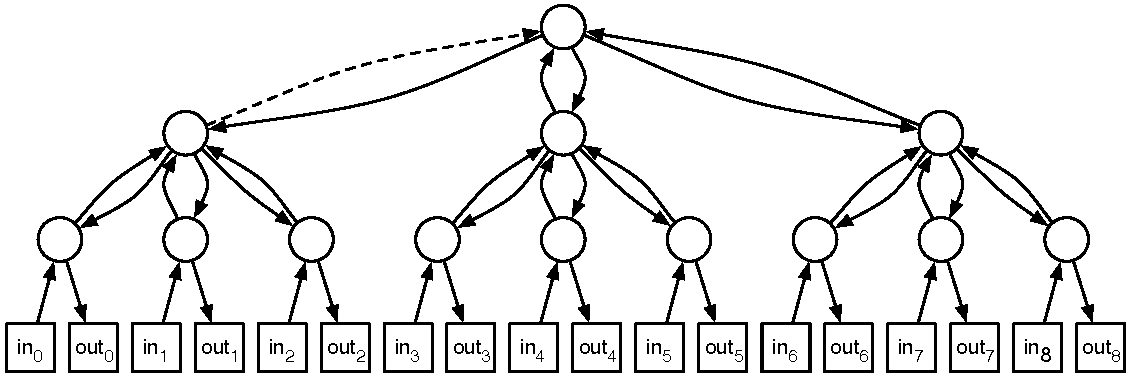
\includegraphics[width=6.5in]{ternary-network}}
\vspace{12pt}

\bparts
%\ppart{??} What is the diameter of this network, including the edges connected to the inputs and outputs? 
%
%\solution[\vspace{0.5in}]{The diameter is the length of the shortest distance between the input and output that are farthest apart. Any path that goes through the top node is a longest path (for example that from $\mathrm{in_0}$ to $\mathrm{out_8}$) with length 6.}

\ppart{10} 
Suppose that each input sends a single packet to an output selected uniformly at random; the packet destinations are mutually independent. (Note that outputs may receive packets from multiple inputs including their corresponding input.)  

What are the expectation and variance of $T$?

\solution[\vspace{1in}]{A packet will pass through the dashed edge if it originates in inputs 0--2 and is destined for outputs 3--8.  For $j \in \{0,1,2\}$ Let $I_j$ be an indicator random variable for the event that a packet leaving input $j$ passes through the dashed edge.  The probability of this event is $\frac{2}{3}$. It follows that:

\begin{align*}
T & = I_1 + I_2 + I_3 \\
Ex[T] 
&= Ex[I_1 + I_2 + I_3] \\
&= Ex[I_1] + Ex[I_2] + Ex[I_3] \\
&= 3\cdot\frac{2}{3} \\
&= 2
\end{align*}

Similarity, but the linearity of variance for independent random variables:

\begin{align*}
T & = I_1 + I_2 + I_3 \\
Var[T] 
&= Var[I_1 + I_2 + I_3] \\
&= Var[I_1] + Var[I_2] + Var[I_3] \\
&= 3 \cdot \frac{2}{3} \cdot \left(1-\frac{2}{3}\right) \\
&= \frac{2}{3}
\end{align*}

}

\instatements{\newpage} 
\ppart{5}
Now consider the situation where a permutation of inputs to outputs is chosen uniformly at random; each input sends a packet to a distinct output. What is the expected value of $T$?  Briefly justify your answer.

\solution[\vspace{1in}]{
	Once again, $T = I_1 + I_2 + I_3$.  By linearity of expectation, 
	$\expect{T} = \expect{I_1} + \expect{I_2} + \expect{I_3}$. 
	We know that $\expect{I_i} = 2/3$ still, because each input is equally likely routed to any of the outputs (even when we only restrict ourselves to permutations).  Thus, 
	$\expect{T} = 3*2/3 = 2$.  
}
\eparts
\end{problem}





% Bill's graph probability problem with two graph cycles
% graphics by Nick
\newpage
\begin{problem}{15} \label{graphprob} \ptitle{Connected or Not? That Is the Question}

Suppose we have a simple, undirected graph $G$ with $2n$ vertices and $2n$ edges, where $n \geq 3$.  The graph consists of two disjoint cycles with $n$ edges each.  For example, if $n=6$, the graph would look like this:

\vspace{12pt}
\centerline{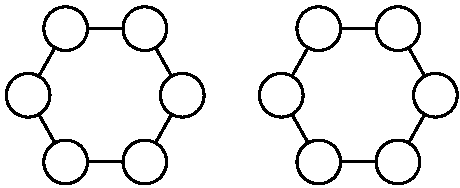
\includegraphics[width=2in]{disconnected-graph}}
\vspace{12pt}

\bparts
\ppart{5}
A pair of vertices $u$ and $v$ from $G$ is selected uniformly at random from the pairs of distinct vertices with no edge between them.  A new graph $G'$ is constructed to be the same as $G$, except that there is an edge between $u$ and $v$.  What is the probability that $G'$ is connected?

\solution[\vspace{2in}]{
$G'$ is connected if and only if $u$ and $v$ come from different cycles.  There are $n^2$ pairs of vertices consisting of vertices in different cycles.  In all, there are ${2n \choose 2} - 2n$ pairs of vertices with no edge between them, since there are ${2n \choose 2}$ pairs of vertices and $2n$ of these pairs have an edge between them.  The desired probability $p$ can be computed as follows:

\begin{eqnarray*}
p & = & \frac{n^2}{{2n \choose 2} - 2n} \\
& = & \frac{n^2}{\frac{2n(2n - 1)}{2} - 2n} \\
& = & \frac{n^2}{2n^2 - n - 2n} \\
& = & \frac{n}{2n - 3}
\end{eqnarray*}
}


\ppart{10} 
$k$ pairs of vertices from $G$ are selected uniformly at random from the pairs of distinct vertices with no edge between them. %, so that each distinct set of $k$ pairs is equally likely to be selected.
 Repetition is allowed; it is possible, for example, that the same pair appears multiple times in the set of $k$ pairs.  A new graph $G''$ is constructed to be the same as $G$, except that there are $k$ new edges: the edges that correspond to the $k$ selected pairs. What is the probability that $G''$ is {\bf not} connected?

%\hint{You may want to verify the consistency between your answers for part (a) and for part (b) for $k=1$.}

\hint{For $k=1$, the sum of your answers to part (a) and part (b) should equal $1$.}

\solution[\vspace{4in}] {
	Note that the probability of not connecting the graph in one sampling of two nonadjacent vertices is
	$$p = 1 - \frac{n}{2n-3}$$
	
	Because we are able to choose the same pair many times, we are simply taking independent samples of two nonadjacent vertices.  Furthermore, in $k$ samples, the graph is not
	connected if and only if none of the pairs chosen have connected the graph.  The probability of this happening is 
	
	$$p^k = (1 - \frac{n}{2n-3})^k$$
}






\eparts
\end{problem}

\renewcommand{\expect}[1]{\operatorname{Ex}[#1]}

\instatements{\newpage}
\begin{problem}{15}\label{chernoff} \ptitle{6.042: The Ultimate Showdown}

There are 100 homework problems in 6.042 throughout the term. Let $T_i$, $1\leq i\leq 100$, be the random variable indicating the fraction of a day that is needed by a student to solve the $i$th problem of 6.042.
 
%For each problem $i$, assume that $0\leq T_i\leq 1$ and $\expect{T_i} =0.3$. 
The distribution for each $T_i$ is different and unknown. We only know that the $T_i$ are mutually independent and that for all $i$, $0\leq T_i\leq 1$ and $\expect{T_i} = 0.3$. 

Let $T$ be the sum of all $T_i$'s; $T$ represents the total number of days needed by a student to complete all homework problems for 6.042. %Use a Chernoff bound to compute an upper bound on the probability that $T\geq e \expect{T}$.
Prove that the probability that $T$ is greater than $30e$ is exceedingly small by deriving the best bound you can on this probability. \hint{We do not consider $1/e$ to be exceedingly small.}

\end{problem}

\solution{
	We know that $T = \sum_i T_i$.  Thus, we know that $\expect{T} = \expect{\sum_i T_i}  = \sum_i \expect{T_i} = 100(.3) = 30$

	Now, from the Chernoff bound (which we can use because the $T_i$ are mutually independent), we have that 
	
	$$Pr\{ T \geq 30e \} \leq e^{-(e - e + 1)\cdot 30} = e^{-30}$$
	
	Which is quite a small bound.

}



% Chieu: (Prob + recurrences) Evolution recurrence problem:
\instatements{\newpage}
\begin{problem}{25}\label{evolution} \ptitle{Gotta Count 'Em All!}

\newcommand{\aaa}{Schemander}
\newcommand{\bbb}{Haskeleon}
\newcommand{\ccc}{Camlizard}

\newcommand{\town}{Functional City}

An unusual species inhabits the forest surrounding \town. Each member of the species can take one of three possible forms, called \emph{\aaa}, \emph{\bbb}, and \emph{\ccc}.

In January of every year, each individual undergoes ``evolution''---a process by which the individual splits into two individuals, whose forms depend on the form of the original:

\begin{itemize}
 \item A \aaa\ splits into a \aaa\ and a \bbb.
 \item A \bbb\ splits into a \aaa\ and a \ccc.
 \item A \ccc\ splits into a \aaa\ and a \bbb.
\end{itemize}

We are investigating the distribution of forms within a large population of this species over time. It is known that in June of year $0$, the population consisted of a single \aaa. %Unfortunately, it is impossible to ``catch 'em all'', so we must use math to figure this out, assuming ideal conditions (
Assume that no individual ever dies and that all individuals successfully undergo evolution exactly once every January.


\bparts

\ppart{3}
Let $S_n$, $H_n$, and $C_n$ be the number of \aaa s, \bbb s, and \ccc s, respectively, in June of year $n$. Express $S_{n}$, $H_{n}$, and $C_{n}$ in terms of $S_{n-1}$, $H_{n-1}$, and $C_{n-1}$, for $n > 0$.

\solution[\vspace{2in}]{
For each form, we look at what forms can be possible parents for it. A \aaa\ can have any of the three forms as a parent, so the number of \aaa s at time $n$ is the number of \aaa s, \bbb s, and \ccc s at time $n-1$. Likewise, a \bbb\ can have either a \aaa\ or a \ccc\ as a parent, and a \ccc\ can have only a \bbb\ as a parent.

Therefore, we can the recurrence equations as
%
\begin{align*}
 S_n &= S_{n-1} + H_{n-1} + C_{n-1} \\
 H_n &= S_{n-1} + C_{n-1} \\
 C_n &= H_{n-1}
\end{align*}
}

\instatements{\newpage}

\ppart5
Let $T_n = S_n + H_n + C_n$ be the total number of individuals in June of year $n$. Use induction to prove that $T_n = 2^n$ for all $n\geq 0$.

\solution[\vspace{5in}]{
We expand each of the three terms using the recurrence:
%
\begin{align*}
 T_n &= S_n + H_n + C_n \\
  &= (S_{n-1} + H_{n-1} + C_{n-1}) + (S_{n-1} + C_{n-1}) + (H_{n-1}) \\
  &=  2(S_{n-1} + H_{n-1} + C_{n-1}) \\
  &= 2(T_{n-1})
\end{align*}
%
We can see that the population doubles every year. Since $T_0 = 1$ (just a single individual), $T_n = 2^n$.
}

\ppart{2}
Show that $H_{n} = T_{n-1} - H_{n-1}$ for $n>0$.

\solution[\vspace{2in}]{
 We use the expression for $H_{n}$ from the recurrence:
%
\begin{align*}
 H_n &= S_{n-1} + C_{n-1} \\
  &= (S_{n-1} + H_{n-1} + C_{n-1}) - H_{n-1} \\
  &= T_{n-1} - H_{n-1} 
\end{align*}
}

\instatements{\newpage}

\ppart{15}
Give a closed-form expression for $H_n$. You may use, without proof, the fact stated in part (b) and the recurrence given in part (c). %(There is more space on the next page.)

\solution{
From parts (b) and (c), we have
%
\begin{align*}
 H_n &= T_{n-1} - H_{n-1} \\
     &= 2^{n-1} - H_{n-1} \\
     &= (1/2)2^n - H_{n-1} \\
 H_n + H_{n-1} &= (1/2)2^n
\end{align*}

This is a linear recurrence. We first solve for the particular solution. Since the $(1/2)2^n$ term is an exponential, we try $f(n) = a2^n$. Plugging this into the recurrence gives us
%
\begin{align*}
 a2^n + a2^{n-1} &= (1/2)2^n \\
 a2^n + (1/2)a2^n &= (1/2)2^n \\
 (3/2)a &= 1/2 \\
 a &= 1/3
\end{align*}

Next we solve for the homogeneous solution:
%
\begin{align*}
 H_n + H_{n-1} &= 0 \\
 r + 1 &= 0 \\
 r &= -1 
\end{align*}
%
So our expression for $H_n$ is of the form
%
\begin{align*}
 H_n &= A(-1)^n + (1/3)2^n 
\end{align*}

We solve for $A$ by using the initial condition $H_0=0$, since there are no \bbb s in year 0.
%
\begin{align*}
 0 &= A(-1)^0 + (1/3)2^0 \\
 &= A + 1/3 \\
 A &= -1/3
\end{align*}

The final expression for $H_n$ is thus
\begin{align*}
 H_n &= (-1/3)(-1)^n + (1/3)2^n
\end{align*}




}


%How many \aaa s are there in the population during year $n$, where $n>0$?

%\ppart{10}

%How many \bbb s are there in the population during year $n$, where $n>0$?

%\hint{Define $S(n)$, $H(n)$, and $O(n)$ as the number of \aaa s, \bbb s, and \ccc s, respectively, during year $n$.}


\eparts

%As $t$ approaches infinity, 
%What is the probability that the single individual is a \aaa after $t$ years?
%a random individual in this population is a \aaa?
%Hint: Define $S(t)$, $H(t)$, and $O(t)$ 
%as the probabilities that the individual is a \aaa, \bbb, and \ccc
% after $t$ years. 

%\solution{For all $t > 0$, the expected proportion of \aaa s in the population is $1/2$, since every individual becomes a \aaa\ with probability $1/2$ every year, regardless of form.}

%\ppart{10} What is the probability that the single individual is a \bbb after $t$ years?
%As $t$ approaches infinity, what is the probability that a random individual in this population is a \bbb?

%\solution{Let $S(t)$ be the proportion of \aaa s, $H(t)$ be the proportion of \bbb s, and $C(t)$ be the proportion of \ccc s at time $t$. Then we can define a recurrence, which holds for $t > 0$:
%\begin{align*}
%S(t) &= \frac12 S(t-1) + \frac12 H(t-1) + \frac12 C(t-1) \\
%H(t) &= \frac12 S(t-1) + \frac12 C(t-1) \\
%C(t) &= \frac12 H(t-1)
%\end{align*}
%We wish to solve for $H(t)$. Since we determined in part (a) that $S(t) = 1/2$ for all $t>0$, $S(t-1) = 1/2$ for all $t>1$. From the recurrence for $C(t)$, we can set $C(t-1) = H(t-2)/2$ for all $t>1$. We then have the following recurrence for $H(t)$, for $t > 1$:

%\begin{align*}
% H(t) &= \frac14 + \frac14 H(t-2) \\
%\end{align*}

%This is a linear recurrence. We first solve for the particular solution, and try $H(t) = c$:

%\begin{align*}
% c &= \frac14 + \frac14 c \\
% \frac34c &= \frac14 \\
% c &= 1/3 \\
%\end{align*}

%Next, we solve for the homogeneous solution. The characteristic equation is

%\begin{align*}
% r^2 - \frac14 &= 0
%\end{align*}

%The solutions are $r = 1/2$ and $r = -1/2$. Our solution is of the form

%\begin{align*}
% H(t) &= A(1/2)^t + B(-1/2)^t + 1/3
%\end{align*}

%Plugging in our initial conditions for $t =0$ and $t=1$, we have

%\begin{align*}
% H(0) = 0 &= A(1/2)^0 + B(-1/2)^0 + 1/3\\
% &= A + B + 1/3 \\
%H(1) = 1/2 &= A(1/2)^1 + B(-1/2)^1 +1/3\\
% &= A/2 - B/2 + 1/3 \\
%\end{align*}

%Solving this system of equations, we get $A = 0$ and $B = 1/3$. Therefore,

%\begin{align*}
% H(t) = \frac13\left(-\frac12\right)^t + \frac13 
%\end{align*}

%Taking the limit as $t\to\infty$, the exponential term converges to $0$, so we are left with $1/3$.}

%\eparts

%\instatements{
%\newpage
%{\bf Room for Problem \ref{evolution}...}
%}


\end{problem}


 
%Chieu: order of growth
\instatements{\newpage}
\begin{problem}{15}\label{orders} \ptitle{Asymptotic Awesomeness}
% Consider the set of order-of-growth relations $R = \{\Theta,O,o,\Omega,\omega\}$. For the following subsets of $R$, determine if there exist functions $f$ and $g$  such that each relation in the subset, and no other relation in $R$, holds between $f$ and $g$. For example, (a) asks if there exist a pair of functions $f$ and $g$ such that $f=\Theta(g)$, $f=O(g)$, and $f=o(g)$, but  $f\not=\Omega(g)$ and $f\not=\omega(g)$. In each case, identify such a pair of functions if they exist.

% \bparts

%\ppart5 $\{\Theta, O, o\}$

%\ppart5 $\{\Omega, \omega\}$

%\ppart5 $\{o\}$

%\ppart5 $\{\Theta, O, \Omega\}$

%\ppart5 $\{O\}$ (tricky)

%\ppart5 $\{\}$ (tricky)

% \eparts

For each row in the following table, determine whether there exist functions $f$ and $g$ that satisfy all the properties marked \textbf{Yes} and do \emph{not} satisfy the properties marked \textbf{No}. You do not have to provide examples.

\begin{center}
\begin{table}[h!b!p!c!]
\newcommand\T{\rule{0pt}{3.6ex}}
\newcommand\B{\rule[-2.2ex]{0pt}{0pt}}

\begin{center}
\begin{tabular}{|c|c|c|c|c|c|c|}
 \hline
\T\B  & $f=\Theta(g)$ & $f=O(g)$ & $f=o(g)$ & $f=\Omega(g)$ & $f=\omega(g)$ & Do $f,g$ exist?\\
 \hline\hline
\T\B \textbf{(a)} &Yes & Yes & Yes & No & No & \insolutions{\textbf{No}}\\
\hline
\T\B \textbf{(b)} &No & No & No & Yes & Yes & \insolutions{\textbf{Yes}}\\
\hline
\T\B \textbf{(c)} &No & No & Yes & No & No & \insolutions{\textbf{No}}\\
\hline
\T\B \textbf{(d)} &Yes & Yes & No & Yes & No & \insolutions{\textbf{Yes}}\\
\hline
\T\B \textbf{(e)} &No & Yes & No & No & No & \insolutions{\textbf{Yes}}\\
\hline
\T\B \textbf{(f)} &No & No & No & No & No & \insolutions{\textbf{Yes}}\\
\hline
\end{tabular}
\end{center}
\end{table}
\end{center}

%\solution{No; Yes; No; Yes; Yes; Yes}
\solution{

\newcounter{Lcount}

 \begin{list}{\textbf{(\alph{Lcount})}}
    {\usecounter{Lcount}
  %    set rightmargin equal to leftmargin
    \setlength{\rightmargin}{\leftmargin}}
  %    we can now begin the "items"

  \item No. $f=\Theta(g)$ implies that $f=\Omega(g)$.
  \item Yes. Example: $f(n) = n^2$; $g(n) = n$.
  \item No. $f=o(g)$ implies that $f=O(g)$.
  \item Yes. Example: $f(n) = n$; $g(n) = 2n$.
  \item Yes. Example: $f(n) = n^2$; $g(n) = n^{(-1)^n + 1}$.
  \item Yes. Example: $f(n) = n^{(-1)^{n+1} + 1}$; $g(n) = n^{(-1)^n + 1}$.
  \end{list}


}

\end{problem}






%Graphs
\instatements{\newpage}
\begin{problem}{20}\label{graphcycle} \ptitle{Yet Another Graph Proof}

 Prove that in a finite directed graph, if every node has at least one outgoing edge, then the graph has a cycle.

\hint{Consider the longest path.}


\solution{
Suppose that every node has at least one outgoing edge. 
Since the digraph is finite, there exists a longest path 
$v_1\rightarrow v_2 \rightarrow \ldots \rightarrow v_h$. Node $v_h$ has an outgoing edge $v_h\rightarrow v$. If $v\not\in \{v_1, v_2, \ldots, v_h\}$, then $v_1\rightarrow v_2 \rightarrow \ldots \rightarrow v_h \rightarrow v$ is a longer path of length $h+1$. Therefore, $v\in \{v_1, v_2, \ldots, v_h\}$, that is, $v=v_i$ for some $1\leq i\leq h$. This means that the graph has a cycle
$v_i\rightarrow \ldots \rightarrow v_h\rightarrow v_i$. 
} 
\end{problem}





% SAME PROBLEM AS QUIZ 1 - but we will change from rotating 4 tiles to rotating 5 tiles 
%
\instatements{\newpage}
\begin{problem}{20}\label{slipped_disc} \ptitle{Revenge of the Slipped Disc Puzzle\texttrademark: The Curse of 6.042}

(This problem is similar to the Slipped Disc Puzzle\texttrademark\ of Quiz 1, but here we rotate 5 tiles instead of 4.)

The Super Awesome Extreme zomgroflolwut Spifftastic-to-the-Max Slipped Disc Puzzle\texttrademark\ consists of a track holding 9 
circular tiles. In the middle is a disc that can slide left and right 
and rotate 
$180^{\circ}$
to change the positions of \emph{exactly} {\bf five} tiles. As shown below, 
there are 
three ways to manipulate the puzzle:

\begin{description}
\item[Shift Right:] The center disc is moved one unit to the right (if there is space).
\item[Rotate Disc:] The {\bf five} tiles in the center disc are reversed.
\item[Shift Left:] The center disc is moved one unit to the left (if there is space).
\end{description} 

\begin{center}
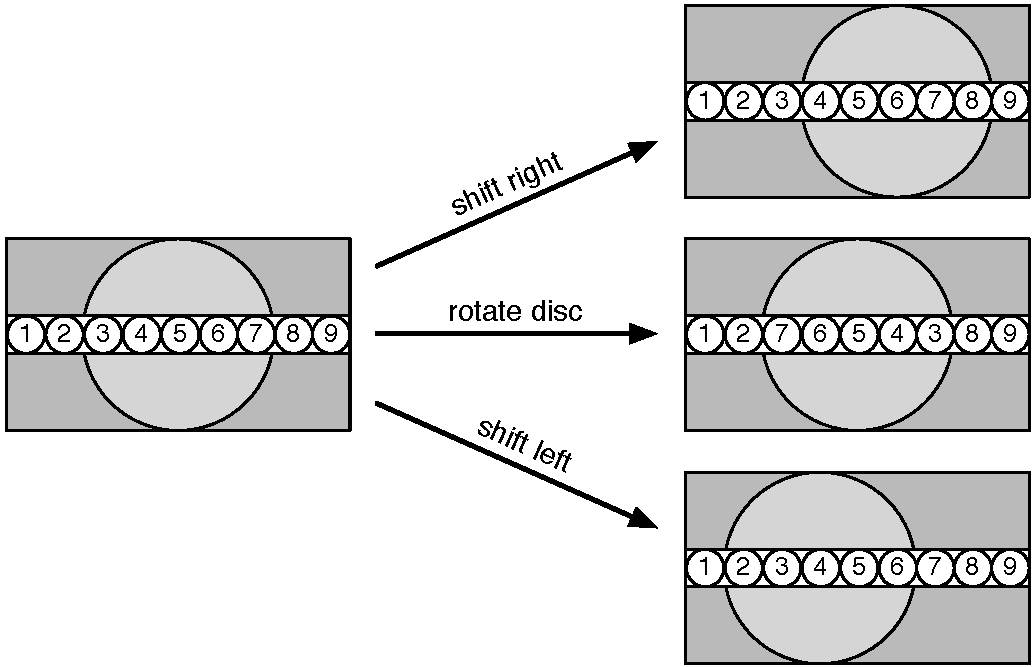
\includegraphics[width=5in]{1d-puzzle-transitions-5slider.pdf}
\end{center}

Prove that if the puzzle starts in an initial state with all but tiles 1 
and 2 in their natural order, then it is impossible to reach a goal state 
where all the tiles are in their natural order.  The initial and goal states are shown below:

\begin{center}
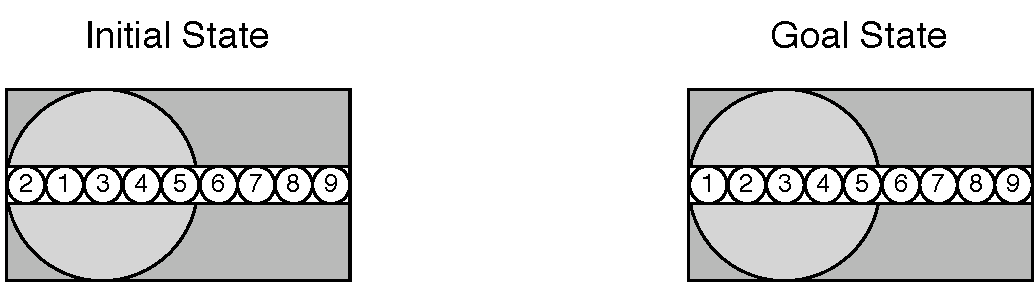
\includegraphics[width=5in]{1d-puzzle-challenge-5slider.pdf}
\end{center}

Write your proof on the next page...

\solution[\newpage]{
Order the tiles from left to right in the puzzle. Define an \emph{inversion} to be a pair of tiles that is out of their natural order (e.g. 4 appearing to the left of 3). 
\begin{lemma*}
Starting from the initial state there is an odd number of inversions after any number of transitions.
\end{lemma*}
\begin{proof}
The proof is by induction.  Let $P(n)$ be the proposition that starting from the initial state there is an odd number of inversions after $n$ transitions.

{\bf Base case:} After 0 transitions, there is one inversion, so $P(0)$ 
holds.

{\bf Inductive step:} Assume $P(n)$ is true.  Say we have a configuration 
that is reachable after $n + 1$ transitions.
\begin{enumerate}
\item Case 1: The last transition was a shift left or shift right

In this case, the left-to-right order of the discs does not change and thus the number of inversions remains the same as in 

\item The last transition was a rotate disc.

In this case, six pairs of disks switch order.  If there were $x$ inversions among these pairs after $n$ transitions, there will be $6 - x$ inversions after the reversal. If $x$ is odd, $6-x$ is odd, so after $n+1$ transitions the number of inversions is odd.
\end{enumerate}
\end{proof}

Conclusion: Since all reachable states have an odd number of inversions and the goal state has an even number of inversions (specifically 0), the goal state cannot be reached.
}

\instatements{
\newpage
{\bf Room for Problem \ref{slipped_disc}...}
}

\end{problem}





\end{document}



%%%%%%%%%%%%%%%%%%%%%%%%%%%DISCARDED%%%%%%%%%%%%%%%%%%%%%%%%%%%
%%%%%%%%%%%%%%%%%%%%%%%%%%%%%%%%%%%%%%%%%%%%%%%%%%%%%%%%%%%%%%%

\iffalse
% Chieu: (Pure probability) Expectation problem: Expected value of expression (depending on student's choices) is student's expected score
\instatements{\newpage}
\begin{problem}{10}\label{radiator}

Let $X$ be the person whose name is written on page 1 of this packet. At the moment, $X$ is attempting to complete Problem \theproblemthm\ of the final exam for a course known as 6.042. The instructions for this problem are self-referential, and $X$ is quite amused by this fact. $X$ is even further amused to find their own amusement acknowledged by the problem statement. It is possible that $X$ even chuckles out loud, much to the annoyance of their fellow test-takers.

The problem statement informs $X$ that the 6.042 course staff have decided to revise their policy for grading the final from the version presented in recitation. A preliminary version of the new policy, however, has apparently upset the radiator behind which some of the finals were to be accidentally dropped under the old policy. The radiator is outraged at the prospect of not having any finals to grade and has demanded a say in $X$'s grades.

To address this concern, the course staff have decided to allow the radiator to grade Problem \theproblemthm\ of the final. The radiator has decided upon the following deterministic algorithm for grading this problem:

It defines a few random variables whose distributions are determined by $X$. Then it computes $T$ ... The expected value of $T$ is then the score $X$ should expect.

After reading the instructions, $X$ decides to select a distribution for each random variable that the radiator requests. $X$ indicates their choice for each random variable by placing a check mark in the appropriate box. 
\end{problem}
\fi


\iffalse
% Spyros: (Counting) 
\instatements{\newpage}
\begin{problem}{??}\label{counting}

Suppose that r flags of different colors are to be displayed on n
distinct poles in a row. An arrangement consists of a selection of which
flags are on which pole, and in which order. A pole can be left without
a flag. How many different arrangements are there?

\solution{The arrangement can be determined by placing one flag after
another. For the first flag, we choose one of the n poles. This pole is
thus divided into two segments, and there are n + 1 possible choices for
the second flag. Similarly, there are n + 2 choices for the third flag.
It follows that there are n * (n + 1) ... * (n + r - 1) possible arrangements.}

\end{problem}
\fi


\iffalse
% Spyros: (Indicator RVs and Expectation) 
\instatements{\newpage}
\begin{problem}{??}\label{indicatorexp}

A 4-sided die has its four faces labeled as a, b, c, d. Each time the die is rolled, the result is a, b, c, or d, with probabilities $p_a, p_b, p_c, p_d$, respectively. Different rolls are statistically independent. The die is rolled n times. Let $N_a$ and $N_b$ be the number of rolls that resulted in a or b, respectively. Define the covariance of two random variables X, Y to be E[X*Y] - E[X]*E[Y]. Find the covariance of $N_a$ and $N_b$. Hint: Use indicator random variables.

\solution{}

\end{problem}
\fi

\iffalse
%Induction
\instatements{\newpage}
\begin{problem}{??}
For $n\geq 1$, let $a_n$ be the largest odd divisor of $n$.  For example, the largest odd divisor of an odd number is the odd number itself, therefore, $a_{2n+1}=2n+1$. Since the largest odd divisor of $2n$ is equal to the largest odd divisor of $n$, $a_{2n}=a_n$.

For $n\geq 0$, let $b_n = a_1+a_2+ \ldots +a_{2^n}$. Prove the equality
$$b_n=\frac{2^{2n}+2}{3}.$$
Hint: $1+3+5+\cdots+(2^{n+1}-1)=2^{2n}$.

\solution{
We use induction. Let $P(n)$, for $n\geq 0$, be the predicate $b_n=\frac{2^{2n}+2}{3}$.

{\bf Base case:}  
$b_0=a_1=1\geq (2^{2\cdot 0}+2)/3$. 

{\bf Inductive step:} Let $n\geq 0$. For the purposes of proving $P(n+1)$, assume $P(n)$. We derive:
\begin{eqnarray*}
b_{n+1} &=& (a_1 + a_3 + \ldots + a_{2^{n+1}-1}) + (a_2 + a_4 +\ldots +a_{2^{n+1}}) \\
&=& 1 + 3+\ldots +(2^{n+1} -1) + (a_1 + a_2 + \ldots +a_{2^n}) \\
&=& 2^{2n} + b_n \\
&\geq & 2^{2n}  + (2^{2n} + 2)/3 
\mbox{ (by the inductive hypothesis $P(n)$)} \\
&=& (2^{2(n+1)} + 2)/3.
\end{eqnarray*}
}
\end{problem}
\fi

\iffalse
%Number theory
\instatements{\newpage}
\begin{problem}{20}
 For integers $n$, $m$, $a$ and $b$, prove that 
$(ma+nb)^k\equiv (ma)^k+(nb)^k \mbox{ (mod } mn)$ for $k\geq 1$.
Hint: Use either the Binomial Theorem or a proof by induction on $k$.
\end{problem}
\fi


\iffalse
%%%%%%%%%%%%%%%%%%%%%%%%%%%
\instatements{\newpage}
\begin{problem}{15} Let $X$ be a non-negative integer random variable and let $a>0$. 
Prove $\pr{X\geq a} \leq \frac{\expect{X^3}}{a^3}$.

\solution{ $\pr{X\geq a}=\pr{X^3\geq a^3} \leq \frac{\expect{X^3}}{a^3}$ by the Markov bound.}

\end{problem}
\fi

\iffalse
\instatements{\newpage}
\begin{problem}{15} compute gcd
\end{problem}
\fi

% Chieu: Implement the Y combinator in PostScript.
\instatements{\newpage}
\begin{problem}{0}\label{postscript}

The Y combinator allows for recursion without defining names for functions. In Scheme, the Y combinator can be expressed as follows:

\begin{verbatim}
(lambda (f)  
    ((lambda (x) (f (lambda (y) ((x x) y))))
     (lambda (x) (f (lambda (y) ((x x) y))))))
\end{verbatim}


In Python, this is

\begin{verbatim}
(lambda f:  
    (lambda x: f(lambda y: (x(x))(y)))   
    (lambda x: f(lambda y: (x(x))(y)))) 
\end{verbatim}

Since PostScript is the best programming language ever created, give an equivalent expression for the Y combinator in PostScript.


\solution{This is a possible solution. 

\begin{verbatim}
{ [ exch
    { [ exch  
        { dup cvx exec exec }
      aload pop ] cvx }
  aload pop 8 -1 roll
    { cvx exec }
  aload pop ] dup cvx exec }
\end{verbatim}

Answers may vary.
}
\end{problem}


% Chieu: (Combinatorial proof; counting and recurrence) Something similar to the Fibonacci number - Hawaiian CV formula, to be derived by counting and by a recurrence ...
\instatements{\newpage}
\begin{problem}{??}\label{combproof}
 insert something here
\end{problem}

% Chieu: (orders of growth) - determine all consistent subsets of the five order-of-growth relations and give examples for each
\instatements{\newpage}
\begin{problem}{10}\label{orders}
Consider the set of order-of-growth relations $R = \{o, O, \Theta, \Omega, \omega\}$.

This set has 32 subsets. For which of the subsets do there exist functions $f(n)$ and $g(n)$ defined for all real numbers $n>0$ such that $f(n), g(n) > 0$, and the subset completely enumerates the order-of-growth relations that hold between $f(n)$ and $g(n)$? For each of these subsets, give a pair of suitable functions.

For example, if there exist functions $f(n)$ and $g(n)$ such that $f(n)=o(g(n))$, $f(n)=O(g(n))$, and $f(n)=\Theta(g(n))$, but $f(n)\not=\Omega(g(n))$ and $f(n)\not=\omega(g(n))$, then indicate that $\{o,O,\Theta\}$ is a valid subset and give examples for $f(n)$ and $g(n)$.

\solution{

Valid subsets are $\emptyset$, $\{o,O\}$, $\{O\}$, $\{O,\Theta,\Omega\}$, $\{\Omega\}$, and $\{\Omega,\omega\}$.
}

\end{problem}

%Logic&RElations
\instatements{\newpage}
\begin{problem}{15}
We define a  relation $R$ on pairs of the Boolean values $\true$ and $\false$ 
by
$$ (p_1,p_2)R(q_1,q_2) \mbox{ iff } \left[
\begin{array}{ll}
(p_1\vee p_2) \Rightarrow (q_1\vee q_2) & \mbox{ and } \\
(p_1\wedge p_2) \Rightarrow (q_1\wedge q_2) & 
\end{array} \right].$$
For example, since $(\false \vee \true) \Rightarrow (\true \vee \false)$
and $(\false \wedge \true) \Rightarrow (\true \wedge \false)$,
$$(\false,\true)R(\true,\false).$$

\bparts

\ppart{1} Give another couple of pairs of Boolean values $(p_1,p_2)$ and $(q_1,q_2)$ for which $(p_1,p_2)R(q_1,q_2)$.

\solution[\vspace{1.5cm}]{For example, $(\false,\false)R(\true,\true)$.}

\ppart{1} Give a couple of pairs of Boolean values $(p_1,p_2)$ and $(q_1,q_2)$ for which $(p_1,p_2)R(q_1,q_2)$ does not hold.

\solution[\vspace{1.5cm}]{For example, $(\true,\true)R(\false,\false)$.}

For the following parts provide a brief explanation (e.g., by giving a counter example):

\ppart{3} Is $R$ reflexive? 

\solution[\vspace{3cm}]{Yes, $(p_1\vee p_2) \Rightarrow (p_1\vee p_2)$ and $(p_1\wedge p_2) \Rightarrow (p_1\wedge p_2)$.}

\ppart{5} Is $R$ symmetric? 

\solution[\vspace{3cm}]{No, $(\true, \false)R(\true, \true)$ but not $(\true, \true)R(\true, \false)$.}

\ppart{5} Is $R$ antisymmetric? 

\solution{No, $(\true, \false)R(\false,\true)$, $(\false,\true)R(\true,\false)$, and $(\true,\false)\neq (\false,\true)$.
}

%\ppart{4} Is $R$ transitive? 

%\solution{Yes, this follows directly from the transitivity of $\Rightarrow$. If $(p_1\vee p_2) \Rightarrow (q_1\vee q_2)$ and $(q_1\vee q_2) \Rightarrow (z_1\vee z_2)$, then $(p_1\vee p_2) \Rightarrow (z_1\vee z_2)$. If $(p_1\wedge p_2) \Rightarrow (q_1\wedge q_2)$ and $(q_1\wedge q_2) \Rightarrow (z_1\wedge z_2)$, then $(p_1\wedge p_2) \Rightarrow (z_1\wedge z_2)$. So, $(p_1,p_2)R(q_1,q_2)$ and $(q_1,q_2)R(z_1,z_2)$ implies $(p_1,p_2)R(z_1,z_2)$.}

\eparts

\end{problem}

% Spyros: (Counting and Probability) 
\instatements{\newpage}
\begin{problem}{20}\label{countingprob} \ptitle{More Fun with Cards}

Two people, Alyssa P.\ Hacker and Ben Bitdiddle, are distributed 7 cards each from a standard deck (52 cards). The remaining cards are not distributed. All hands are equally likely. 
\bparts

\ppart{10}
Define $C$ to be the event that Alyssa has all four aces or Ben has all four aces. Find the probability of $C$.

\solution[\vspace{2in}]{
}

\ppart{10}
Find the probability that all four aces are distributed between Alyssa and Ben.

\solution{SOLUTION TO BE UPDATED
SOLUTION TO OLD PROBLEM (each person gets 26 cards):
The total number of choices is (52 choose 26). The number of possibilities where the first person receives all four aces is equal to the number of ways to distribute the remaining 48 cards, with 22 going to player 1 and 26 going to payer 2, which is (48 choose 22). Thus, the answer is (48 choose 22) divided by (52 choose 26).}

\eparts

\end{problem}

